\documentclass[UTF8]{article}  %其他文类:book、report、letter

\usepackage{ctex}
\usepackage{xltxtra} % 提供了针对XeTeX的改进并加入了XeTeX的logo
%特殊标志宏包
\usepackage{texnames,mflogo}
\usepackage{graphicx} % 插入图片宏包
\graphicspath{{figures/}} %指定图片在当前目录下的figures目录,可以有多个目录,需用花括号
\usepackage{amsmath} %矩阵
\usepackage[style=numeric,backend=biber]{biblatex} %参考文献
\addbibresource{biblatex.bib} %引用参考文献文件,不能省略后缀名

% 自定义命令
\newcommand\PRC{People's Republic of \emph{China}} %简单的字符串定义
\renewcommand\abstractname{简介}



%opening
\title{Article排版指南}  %文章标题
\author{令平子}  %作者
\date{2019年10月1日} %自定义日期,没有这项则默认为当前日期

\begin{document}

\maketitle   %生成标题
\tableofcontents %产生目录

\begin{abstract}
\noindent	中文编译用:Xe\LaTeX \\
	英文编译用:pdf\LaTeX \\
	% 分段用空行或\par
\par	TeXLive+TeXstudio
	编译中文需要ctex宏包(或者直接引用ctexart文类),并使用UTF8编码格式
	
	运用命令行查看帮助文档,比如texdoc ctex。

\end{abstract}
\section{字体设置}
% 字体族设置(罗马字体、无衬线字体、打字机字体)
\noindent \textrm{Roman Family}  \textsf{Sans Serif Family} \texttt{Typewriter Family}\\%设置字体为罗马字体,单行不缩进
\rmfamily Roman Family %声明后续字体为罗马字体
{\sffamily Sans Serif Family} {\ttfamily Typewriter Family}
\paragraph{中文字体}%需要ctex宏包
{\songti 宋体} \quad {\heiti 黑体} \quad {\fangsong 仿宋}\quad {\kaishu 楷书}

中文字体的\textbf{粗体}与\textit{斜体}
\section{字号设置}
{\tiny Hello}\\
{\scriptsize Hello}\\
{\footnotesize Hello}\\
{\small Hello}\\
{\normalsize Hello}\\
{\large Hello}\\
{\Large Hello}\\
{\LARGE Hello}\\
{\huge Hello}\\
{\Huge Hello}\\
{\zihao{0} 初号}\\
{\zihao{-0} 小初号}\\
{\zihao{1} 一号}\\
{\zihao{-1} 小一号}\\
{\zihao{2} 二号}\\
{\zihao{-2} 小二号}\\
{\zihao{3} 三号}\\
{\zihao{-3} 小三号}\\
{\zihao{4} 四号}\\
{\zihao{-4} 小四号}\\
{\zihao{5} 五号}\\
{\zihao{-5} 小五号}\\
{\zihao{6} 六号}\\
{\zihao{-6} 小六号}\\
{\zihao{7} 七号}\\
{\zihao{8} 八号}\\
\section{篇章结构}
\subsection{小节}


\section{数学公式}
\paragraph{行内公式}夹杂在$\sum_{i=1}^{n} {x^2}$文字中
\paragraph{单行公式}
$$a^2+b^2=c^2$$
需使用自动编号和交叉引用,要使用equation环境。\\
扩展见式\ref{eq:勾股定理}
\begin{equation}
	a^2+b^2=c^2 \label{eq:勾股定理}
\end{equation}

\(3x^{20}+4x=100\)

\[3x+2^20-x^3\]

\section{特殊符号}
\subsection{空白符号}
\noindent 空行分段,多个空行等同1个\\
自动缩进,绝对不能使用空格代替\\
英文中多个空格处理为1个空格,中文中空格将被忽略\\
汉字与其它字符的间距会自动由XeLaTeX处理\\
禁止使用中文全角空格\\
\subsection{空格长度控制}
%1em(当前字体中M的宽度) 
a\quad b \\
%2em
a\qquad b \\
%约为1/6个em
a\,b a\thinspace b \\
%0.5个em
a\enspace b \\
%空格
a\ b \\
%硬空格
a~b \\
%弹性长度
a\hfill b\\
\subsection{\TeX 标志符号}
\TeX{} \LaTeX{} \LaTeXe{}
\XeLaTeX
\subsection{其它宏包中的标志}
\paragraph{texnames宏包}
\AmSTeX{} \AmS-\LaTeX{} \BibTeX{} \LuaTeX{}
\paragraph{mflogo宏包}
\METAFONT{} \MF{} \MP{}

\paragraph{连字符}
- -- --- ----
\subsection{矩阵}
需要引用amsmath数学宏包\\
\[
\begin{matrix}
0 & 1 \\
1 & 0 
\end{matrix}
\]
\section{插入图片}
使用graphicx宏包

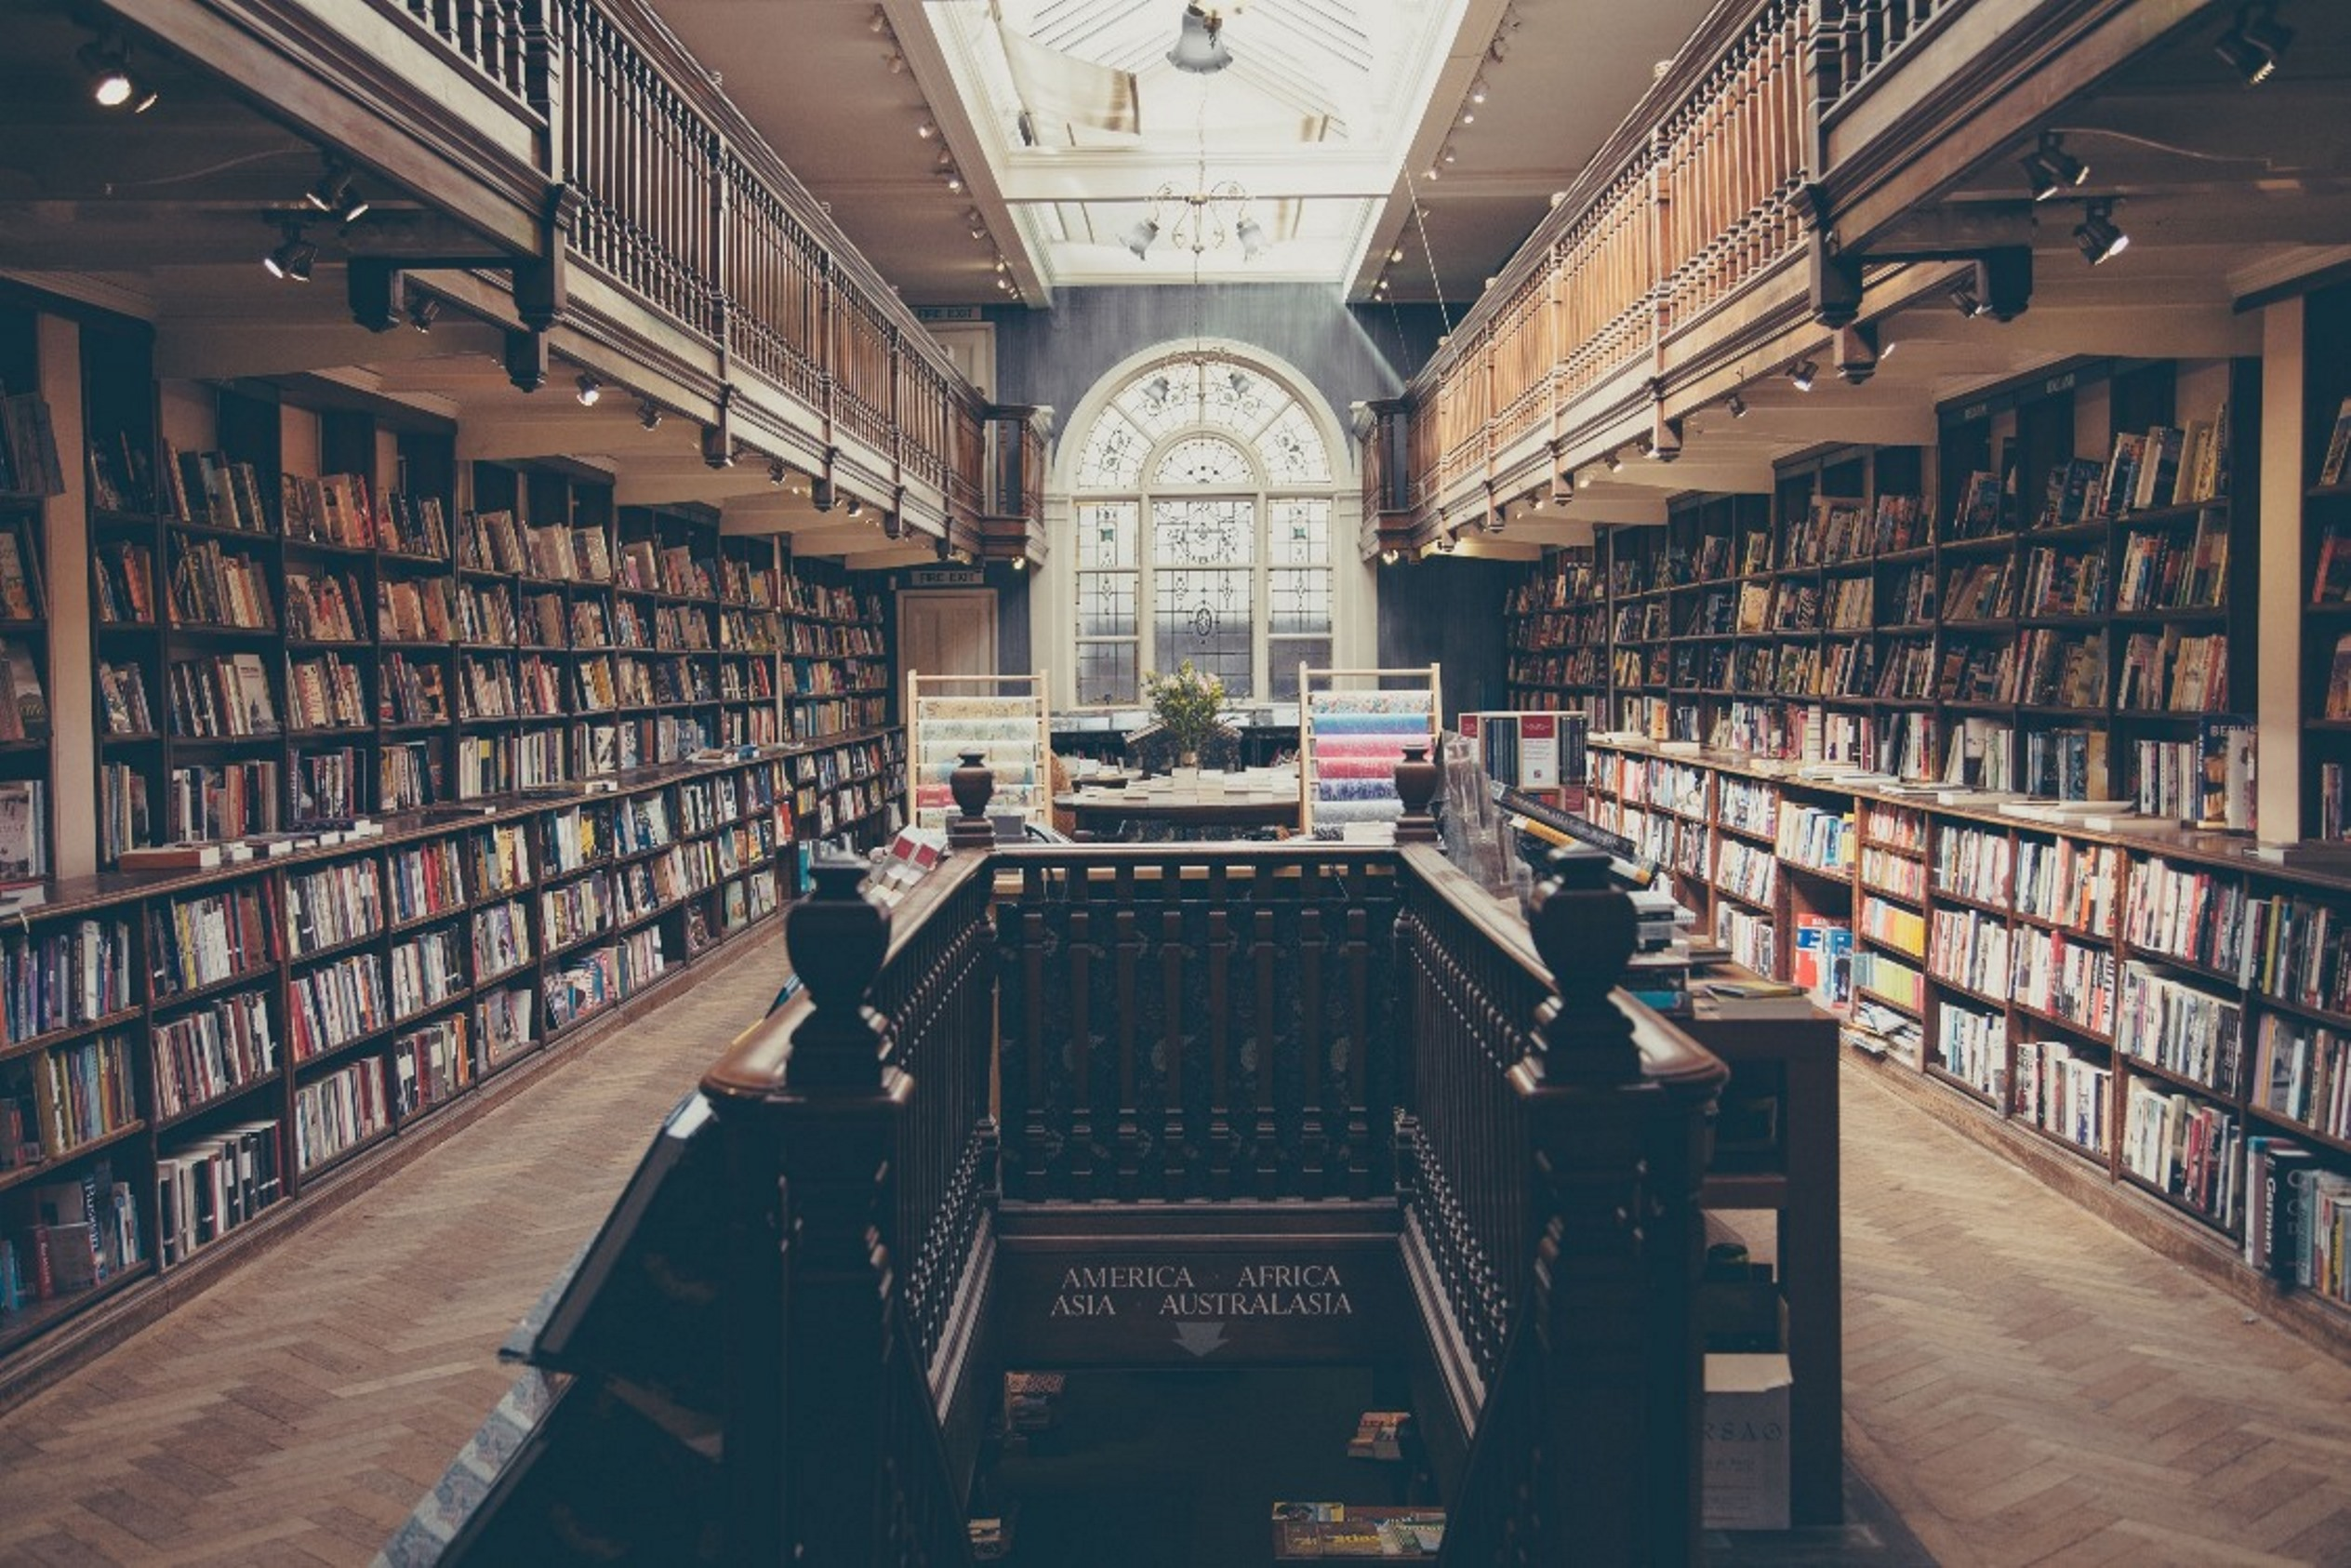
\includegraphics[scale=0.1]{library.jpg}

宽度width= ,高度height= ,缩放比例scale= ,旋转角度angle= 。
帮助文档texdoc graphicx
\section{表格制作}
\begin{tabular}{|l||c|c|c|r|} %左对齐、右对齐、居中对齐
	\hline \hline
	姓名 & 语文 & 数学 & 外语 & 备注 \\
	\hline \hline
	张三 & 87 & 100 & 93 & 优秀 \\
	\hline
	李四 & 75 & 64 & 52 & 补考另行通知 \\
	\hline \hline
\end{tabular}
\\

使用竖线产生表格竖线,hline命令产生表格横线,没有则没有网格线。固定本列宽度用 p{1.2cm},可以自动换行。

帮助文档 texdoc booktab、texdoc longtab、texdoc tabu。
\section{浮动体环境}

为了更灵活地插入图表,使用浮动体环境。交叉引用,见图\ref{fig-library}

\begin{figure}[htbp] %允许放置位置
	\centering
	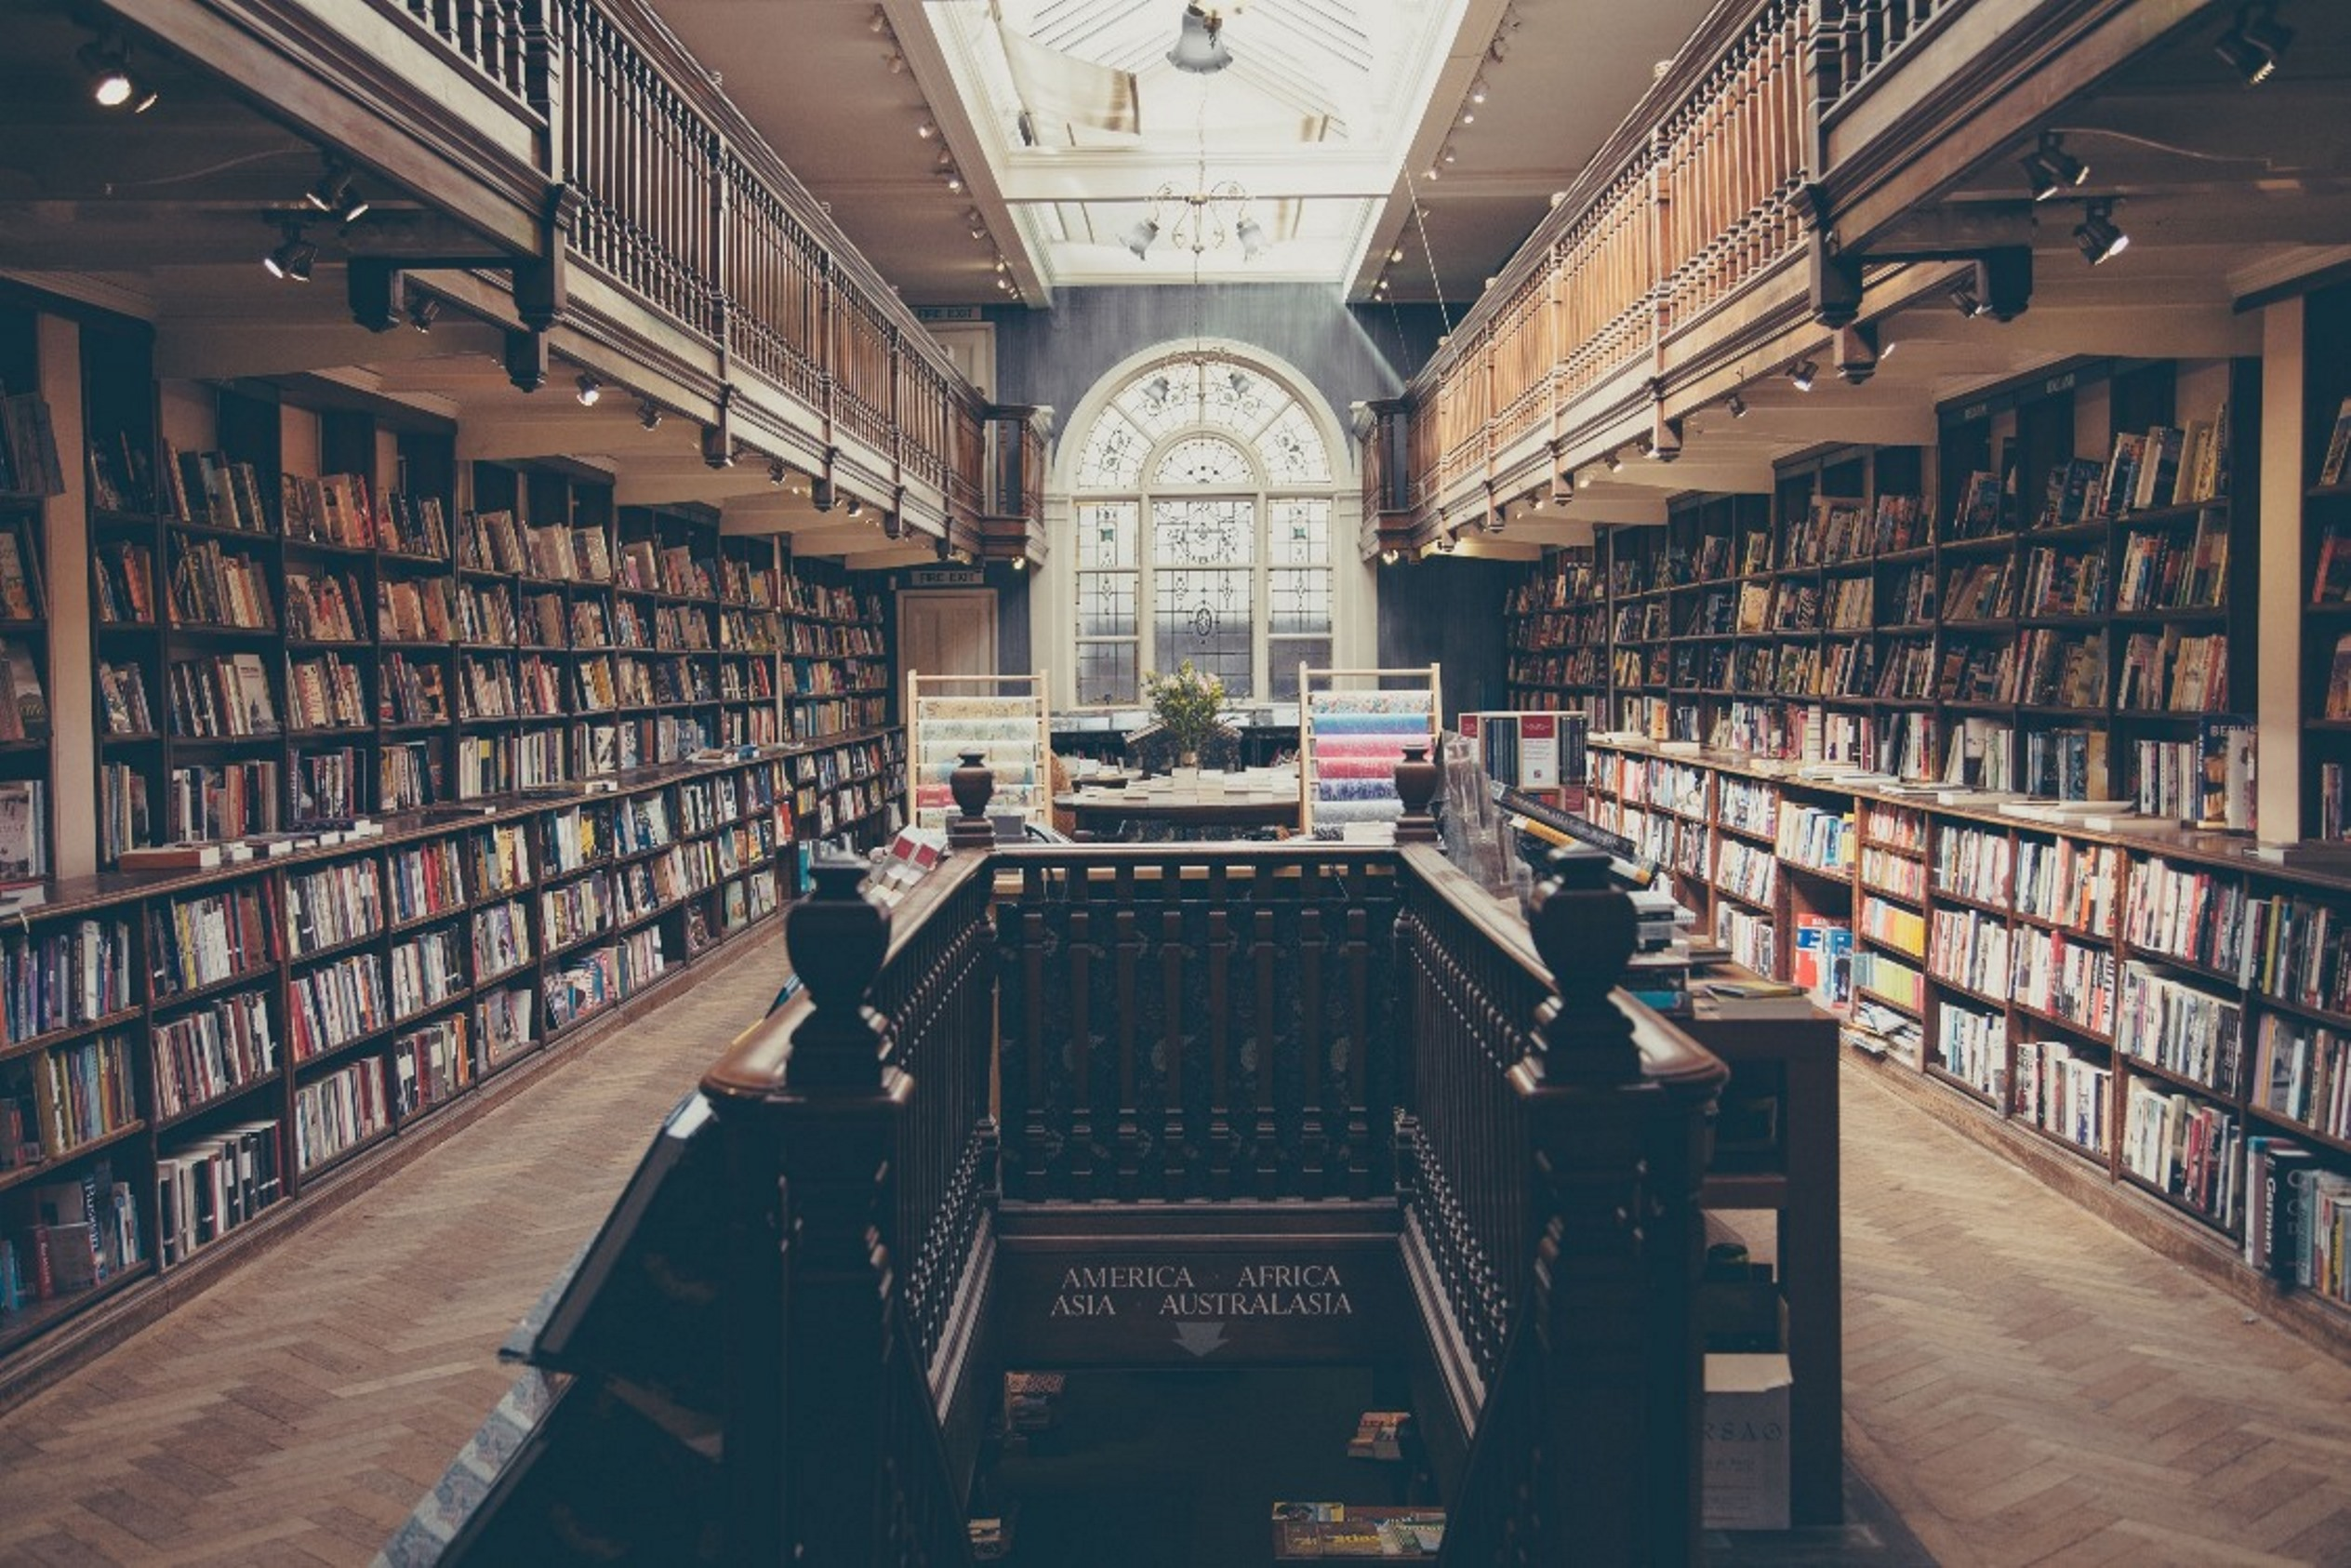
\includegraphics[scale=0.1]{library}
	\caption{图书馆}\label{fig-library}
\end{figure}

本班成绩见表\ref{tab-score}

\begin{table}[htbp]
	\centering
	\caption{成绩单}\label{tab-score}
	\begin{tabular}{|l||c|c|c|r|} %左对齐、右对齐、居中对齐
		\hline \hline
		姓名 & 语文 & 数学 & 外语 & 备注 \\
		\hline \hline
		张三 & 87 & 100 & 93 & 优秀 \\
		\hline
		李四 & 75 & 64 & 52 & 补考另行通知 \\
		\hline \hline
	\end{tabular}
\end{table}

\paragraph{允许位置}
默认tbp\\
h,此处(here)-代码所在的上下文位置\\
t,页顶(top)-代码所在页面或之后页面的顶部\\
b,页底(bottom)-代码所在页面或之后页面的底部\\
p,独立一页(page)-浮动页面

标题控制(caption、bicaption等宏包)\\
并排与子图表(subcaption、subfig、floatrow等宏包)\\
绕排(picinpar、wrapfig等宏包)\\

\section{参考文献BibLaTeX}
 biblatex/biber\\
 新的TEX参考文献排版引擎\\
 样式文件(参考文献样式文件--bbx文件,引用样式文件--cbx文件)使用latex编写\\
 支持根据本地化排版,如:\\
 biber -1 zh pinyin texfile ,用于指定按拼音排序\\
 biber -1 zh stroke texfile ,用于按笔画排序

需要引用biblatex宏包,默认参考文献编译选择biber

参考文献的交叉引用\cite{__2000}

无格式化引用\cite{brown_long-term_2010}

带方括号的引用\parencite{huang_empirical_1998}

上标引用\supercite{perea_topological_2019}

%生成参考文献列表
\nocite{*} %列出所有参考文献,默认列出正文引用的参考文献,开始之前先清理辅助文件
\printbibliography[title={参考文献}] % 默认为英文

\section{自定义命令和环境}
在导言区自定义\\
newcommand用于定义命令\\
命令只能有字母组成,不能以end开头\\
newcommand命令[参数个数(1-9)][首参数默认值]{具体定义}\\%参数个数使用时数字前加#
\PRC

renewcommand重定义命令,用法用自定义命令一致


\end{document}
